\documentclass[10pt,t]{beamer}

\usetheme[progressbar=frametitle,sectionpage=none]{metropolis}

\usepackage{booktabs}
\usepackage[scale=2]{ccicons}

\usepackage{pgfplots}
\usepgfplotslibrary{dateplot}

\usepackage{xspace}
\newcommand{\themename}{\textbf{\textsc{metropolis}}\xspace}

\usepackage{tikz}
\usetikzlibrary{shapes.geometric, arrows}
\tikzset{font=\scriptsize}
\tikzstyle{startstop} = [rectangle, rounded corners, minimum width=2.7cm,%
minimum height=0.6cm, text centered, draw=black, fill=mLightBrown!50]
\tikzstyle{compute} = [rectangle, minimum width = 2.7cm, minimum height = 0.7cm,%
text centered, draw=black, fill=mLightGreen!40]
\tikzstyle{logic} = [diamond, minimum width = 1.2cm,%
text centered, draw=black, fill=mDarkTeal, text=white]
\tikzstyle{data} = [circle, minimum width=0.5cm,text centered,%
draw=black,fill=white]
\tikzstyle{arrow} = [thick,->,>=stealth]
\tikzstyle{line} = [thick]

%% symbols
\newcommand{\bX}{\mathbf{X}}
\newcommand{\bY}{\mathbf{Y}}
\newcommand{\mat}[1]{\mathbf{#1}}
\renewcommand{\vec}[1]{\boldsymbol{#1}}

\title{Real time prediction of bus arrival}
%\subtitle{}
\date{July 31, 2016}
\author{Tom Elliott}
\institute{Supervised by Professor Thomas Lumley\\[2em]

\includegraphics[height=1.5cm]{stat-logo.png}}
%Department of Statistics\\University of Auckland}
%\titlegraphic{\hfill
\includegraphics[height=1.5cm]{stat-logo.png}}

\begin{document}

\maketitle

% \begin{frame}{Table of contents}
%   \setbeamertemplate{section in toc}[sections numbered]
%   \tableofcontents[hideallsubsections]
% \end{frame}

\section{Introduction}

\begin{frame}[fragile]{Overview}
  \onslide<+->
  \begin{enumerate}[<+- | alert@+>]
    \item General Transit Feed Specification (GTFS)

    \item Sequential state space models
      \begin{itemize}[<1->]
        \item Kalman Filter
        \item Particle filter
      \end{itemize}

    \item Predictive models: future arrival times
      \begin{itemize}[<1->]
        \item Schedule
        \item Historical data
        \item Current state
        \item ``Real time'' travel/congestion from other buses
        \item Combinations of the above
      \end{itemize}

    \item Communicating predictive error to commuters

    \item Solving other common problems
  \end{enumerate}
  \onslide<+->
\end{frame}


\section{GTFS}

\begin{frame}{GTFS}
  \onslide<+->
  \begin{itemize}[<+- | alert@+>]
    \item General Transit Feed Specification
      \begin{itemize}
      \item Static schedule information: trips, routes, shapes,
        schedules
      \item GPS location of buses
      \end{itemize}

    \item Standardised by Google and used globally
    \item API provided by Auckland Transport (AT)\\
      \url{https://dev-portal.at.govt.nz}
  \end{itemize}

  \begin{overprint}
    \onslide<5>
    \begin{figure}
      \vspace{-3em}
      \centering
      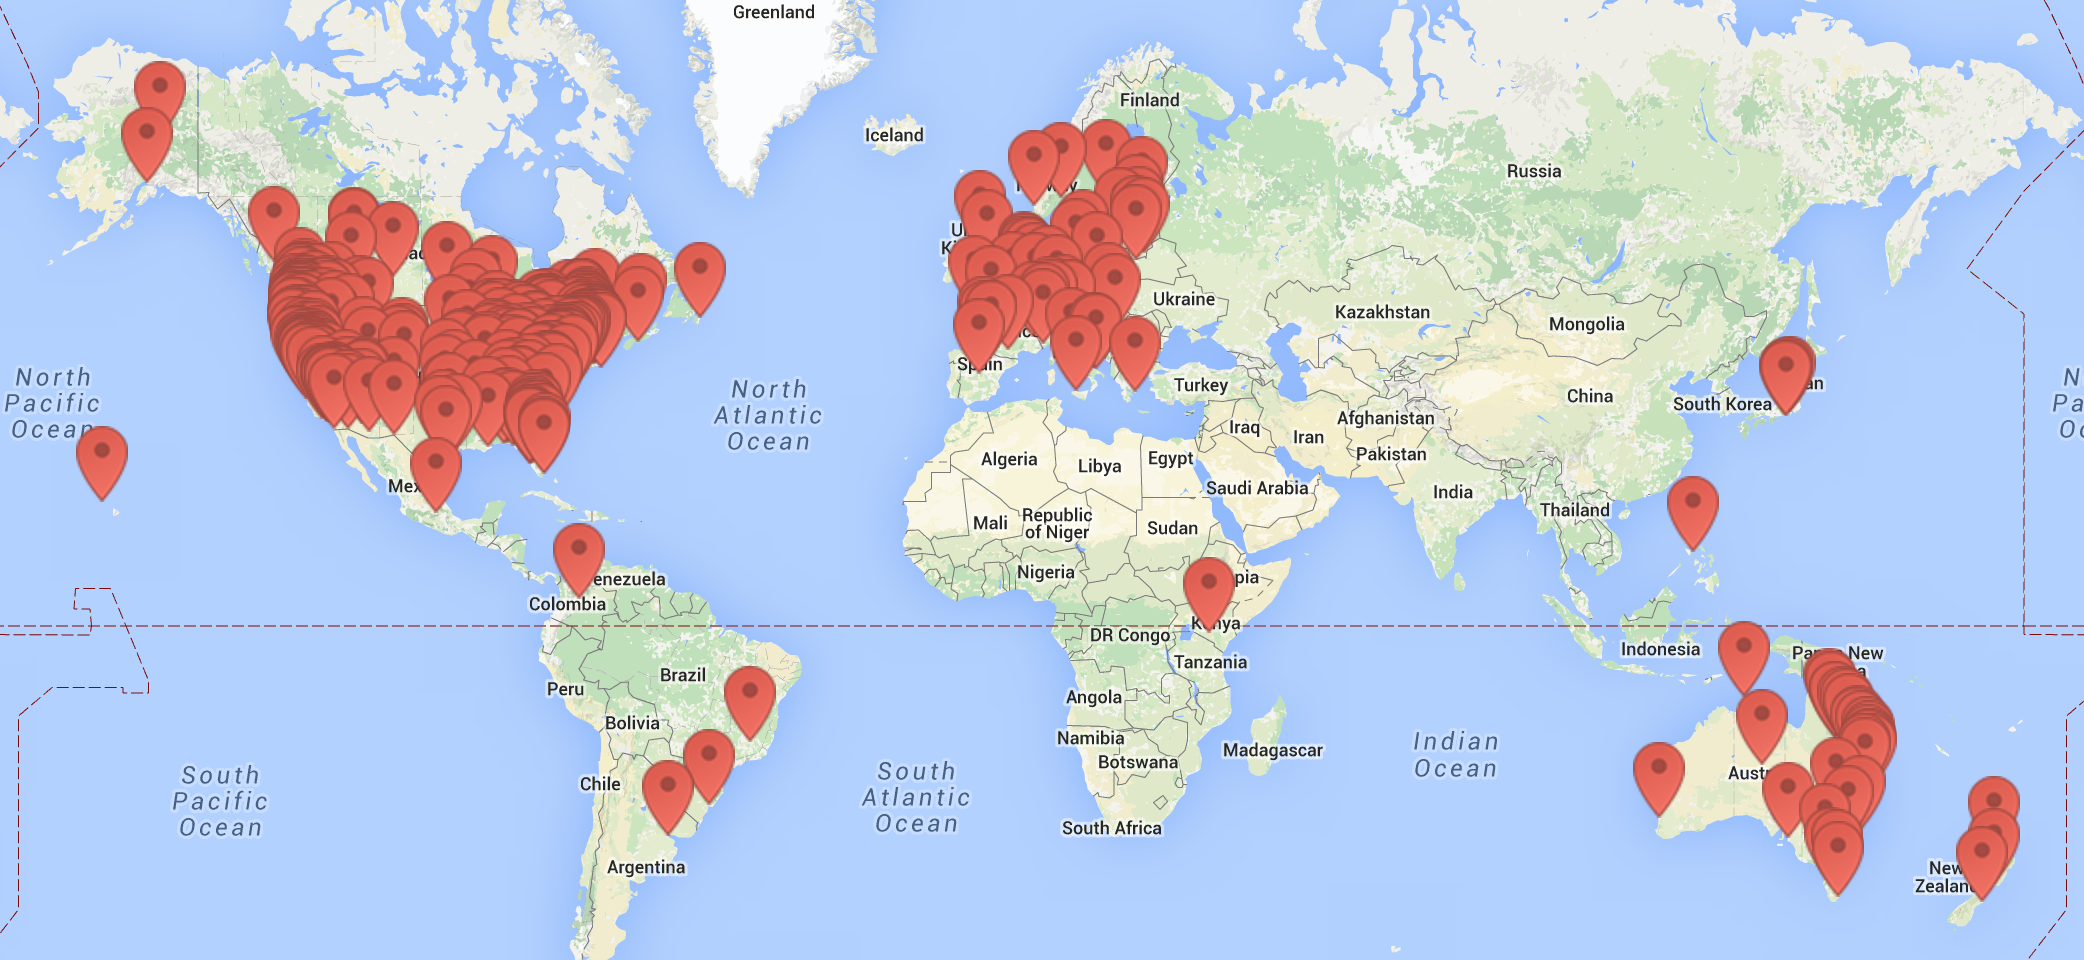
\includegraphics[height=4cm]{gtfs-feeds.png}
      \caption{Global GTFS feeds, \url{http://transitfeeds.com/}}
    \end{figure}
  \end{overprint}
  \onslide<+->
\end{frame}


\section{Modeling Real Time Data}

\begin{frame}{Modeling Real Time Data}
  \onslide<+->
  \begin{itemize}[<+- | alert@+>]
    \item new observations every 30 seconds:
      \begin{equation*}
        \bY_k =
        \begin{bmatrix}
          \phi_k & \lambda_k & t_k
        \end{bmatrix}^T
      \end{equation*}
      $\phi$ = latitude (north/south), $\lambda$ = longitude (east/west)

    \item each observation corresponds to an unknown \emph{state}:
      \begin{equation*}
        \bX_k =
        \begin{bmatrix}
          d_k & v_k & \cdots
        \end{bmatrix}^T
      \end{equation*}
      $d$ = distance into trip (m), $v$ = velocity (speed, m/s)

    \item want to \emph{update} the state of the model from the previous state using the latest observation
      \begin{equation*}
        \bX_k = f(\bX_{k-1}, \bY_k)
      \end{equation*}
  \end{itemize}
  \onslide<+->
\end{frame}

\begin{frame}{Modeling Real Time Data: Kalman Filter I}
  \onslide<+->
  \begin{itemize}[<+- | alert@+>]
    \item Used in robotics, GPS tracking, etc.

    \item Several bus tracking/prediction applications\\
      (Wall \& Dailey (1999), Dailey \emph{et.~al} (2001),
      Cathey \& Dailey, 2004)

    \item Very fast (matrix multiplication), two steps:
      \begin{enumerate}
        \item Predict:
          \begin{equation*}
            \bX_k = \mat{A}_k \bX_{k-1} + \vec{w}_k
          \end{equation*}
          $\mat{A}_k$ depends on $\delta_k$ = time since last observation\\
          $\vec{w}_k$ = Gaussian process noise
        \item Update:
          \begin{equation*}
            \vec{z}_k = \mat{H} \bX_k + \vec{v}_k
          \end{equation*}
          $\mat{H} $ = observation model\\
          $\vec{v}_k$ = Gaussian measurement error\\
          $\vec{z}_k$ = observed data$^\dagger$
      \end{enumerate}
  \end{itemize}
  \onslide<+->
\end{frame}

\begin{frame}{Modeling Real Time Data: Kalman Filter II}
  \onslide<+->
  \begin{itemize}[<+- | alert@+>]
      \item Assumes all errors are normal

      \item Cannot map $\bX_k$ directly to $\bY_k$,
        complicated algorithms to first \emph{estimate} $\vec{z}_k$

      \item All dynamics need to be specified in $\mat{A}_k$\\
        e.g., $d_k = d_{k-1} + v_{k-1}\delta_k + \text{process noise}$
        (Newton's laws of motion)

        \begin{itemize}
        \item not easy to include complex features: e.g., dwell
          times
        \end{itemize}


      \item can't cope with multi-modal posterior:
        \begin{itemize}[<1->]
          \item loops
          \item delays/detours
        \end{itemize}

      \item posterior is (multivariate) normal
  \end{itemize}
  \onslide<+->
\end{frame}


\section{Particle Filter}

\begin{frame}{Modeling Real Time Data: Particle Filter I}
  \onslide<+->
  \begin{itemize}[<+- | alert@+>]
    \item Generalises almost everything from KF

    \item Simulates ``imaginary'' buses with state $\bX_k^{(i)}$

    \item Predict each particle to generate \emph{prior distribution}:
      \begin{equation*}
        \tilde\bX_k^{(i)} = f(\bX_{k-1}^{(i)}, \sigma_v^2)
      \end{equation*}
      No restrictions on $f$ (except computational)

    \item Resample particles based on observed GPS coordinates:
      \begin{equation*}
        w_1^{(i)} = \frac{p(\bY_k | \tilde\bX_k^{(i)})}{\sum_{j=1}^M p(\bY_k | \tilde\bX_k^{(j)})}
      \end{equation*}
      $p(y,x)$ is the \emph{likelihood}

    \item New sample is the \emph{posterior distribution} of $\bX_k$
  \end{itemize}
  \onslide<+->
\end{frame}


\begin{frame}{Modeling Real Time Data: Particle Filter II}
  A simple example using only one dimension (distance).

  \onslide<+->

  \begin{itemize}[<+- | alert@+>]
    \item Start with previous state $\bX_{k-1}$
    \item Use model to predict state $\tilde\bX_{k}$
    \item Add process noise
    \item Get observation $\bY_k$
    \item Compute weights based on distance from observation
    \item Weighted resample to get $\bX_k$
  \end{itemize}
  %\vspace{5cm}
  \begin{overprint}
    \onslide<2>
    \centering
    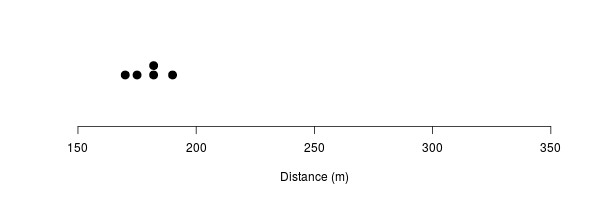
\includegraphics[width=0.8\textwidth]{figs/pf1-frame1.png}
    \onslide<3>
    \centering
    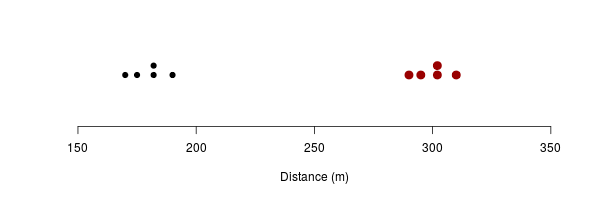
\includegraphics[width=0.8\textwidth]{figs/pf1-frame2.png}
    \onslide<4>
    \centering
    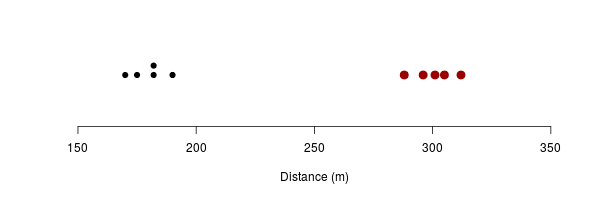
\includegraphics[width=0.8\textwidth]{figs/pf1-frame3.png}
    \onslide<5>
    \centering
    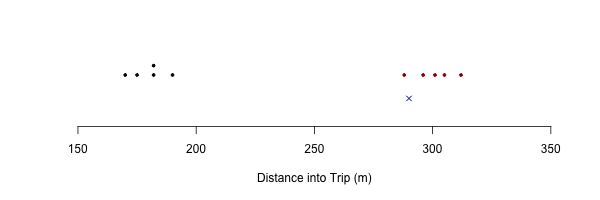
\includegraphics[width=0.8\textwidth]{figs/pf1-frame4.png}
    \onslide<6>
    \centering
    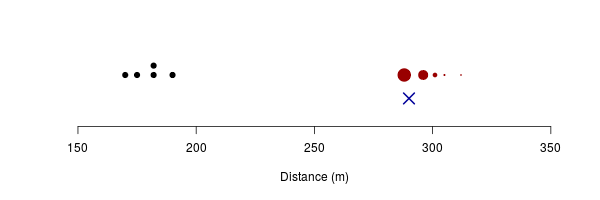
\includegraphics[width=0.8\textwidth]{figs/pf1-frame5.png}
    \onslide<7->
    \centering
    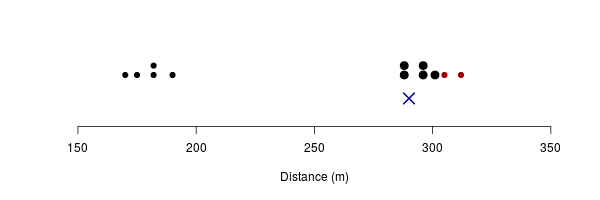
\includegraphics[width=0.8\textwidth]{figs/pf1-frame6.png}
  \end{overprint}
  \onslide<+->
\end{frame}


\begin{frame}{Modeling Real Time Data: Model I}
  \onslide<+->
  \begin{itemize}[<+- | alert@+>]
    \item Newton's Laws of Motion
      \begin{itemize}[<1->]
        \item Model dynamic motion of vehicles with time\\
          $d_k = d_{k-1} + \delta_k v_{k}$, $v_k = v_{k-1} + \text{noise}$
        \item Not good for buses stopping frequently for passengers
      \end{itemize}

    \item Bus behaviour
      \begin{itemize}
        \item Follow motion laws between stops
        \item Stop at bus stop $j$ with probability $\pi_j$
        \item If bus stops:
          \begin{itemize}[<1->]
            \item decelerate and open doors
            \item allow passengers to alight and embark
            \item close doors and accelerate
          \end{itemize}
        \item If bus doesn't stop, do none of the above
        \item Traffic lights: just use a very small ``$\pi$''
          that works in almost the same way
      \end{itemize}
  \end{itemize}
  \onslide<+->
\end{frame}

\begin{frame}{Modeling Real Time Data: Model II}
  \onslide<+->
  \begin{itemize}[<+- | alert@+>]
    \item Dwell time at stop $j$
      \begin{itemize}
        \item Given a bus stops \ldots
        \item it will always decelerate,
          open/close doors, and accelerate: $\gamma$
        \item it will then wait at the bus stop until passengers
          have alighted/boarded: $\tau_j \sim \mathcal{E}(\mu_\tau)$
        \item Total travel time lost at bus stop = dwell time
      \end{itemize}

    \item Particle filter model
      \begin{itemize}
        \item Just include logic in $f$
        \item $p_j^{(i)} \sim \text{Bernoulli}(\pi_j)$
        \item if $p_j^{(i)} = 1$, then \ldots\\
          \ldots wait at stop for $\gamma + \tau_j^{(i)}$~seconds before continuing
      \end{itemize}
  \end{itemize}
  \onslide<+->
\end{frame}

\begin{frame}{Modeling Real Time Data: Model III}
  Particle Filter model, $\bX_k = f(\bX_{k-1}, \bY_k, \sigma_v, \sigma_y)$

  \vspace{0.5cm}
  \begin{tikzpicture}[node distance=1.4cm]
    \node (start) [startstop] {Previous State, $\bX_{k-1}$};
    \node (move) [compute, below of=start,align=center] {Add noise, $\sigma_v$\\ Move Forward};
    \node (stateEst) [startstop, below of=move] {Estimated State, $\tilde\bX_k$};
    \node (resample) [compute, below of=stateEst,align=center] %
    {Compute likelihood, $\sigma_y$\\Weighted Resample};
    \node (end) [startstop, below of=resample] {Final State, $\bX_k$};

    \node (data) [data, right of=resample, xshift=1cm] {$\bY_k$};

    \onslide<2->{\node (passStop) [logic, right of=move, xshift=1.5cm] {\tiny Pass stop?};
    \node (arrival) [compute, right of=passStop, xshift=1.5cm, align=center]%
      {Get arrival time\\ Sample $p \sim \text{Bern}(\pi)$\\%
      Sample $\tau \sim \mathcal{E}(\mu_\tau)$};
    \node (remaining) [logic, right of=arrival, xshift=1.5cm] {\tiny Time left?};
    \node (moveForward) [compute, above of=arrival, align=center]%
      {Get departure time\\Move forward};
    \node (stopped) [compute, below of=arrival] {Position at stop};
    }

    \draw [arrow] (start) -- (move);
    \draw [arrow] (stateEst) -- (resample);
    \draw [arrow] (data) -- (resample);
    \draw [arrow] (resample) -- (end);
    \onslide<1>\draw [arrow] (move) -- (stateEst);
    \onslide<2->\draw [arrow] (move) -- (passStop);

    \draw [arrow] (passStop) -- node[anchor=south] {yes} (arrival);
    \draw [arrow] (arrival) -- (remaining);
    \draw [arrow] (remaining) |- node[anchor=west] {yes} (moveForward);
    \draw [arrow] (moveForward) -| (passStop);
    \draw [arrow] (remaining) |- node[anchor=west] {no} (stopped);
    \draw [arrow] (stopped) -- coordinate[midway] (toEst) (stateEst);
    \draw [line] (passStop) -- node[anchor=west] {no} (toEst);
  \end{tikzpicture}
\end{frame}

\begin{frame}{Modeling Real Time Data: Example}
  \begin{itemize}
    \item Applied to data collected from a bus route
    \item Non-informative priors (speed, dwell times, stopping probabilities)
    \item \emph{Always} a small probability of not moving (e.g., traffic lights)
  \end{itemize}
\end{frame}

{ % all template changes are local to this group.
    \setbeamercolor{background canvas}{bg=white}
    \begin{frame}[plain]
        \begin{tikzpicture}[remember picture,overlay]
            \node[at=(current page.center)] {
                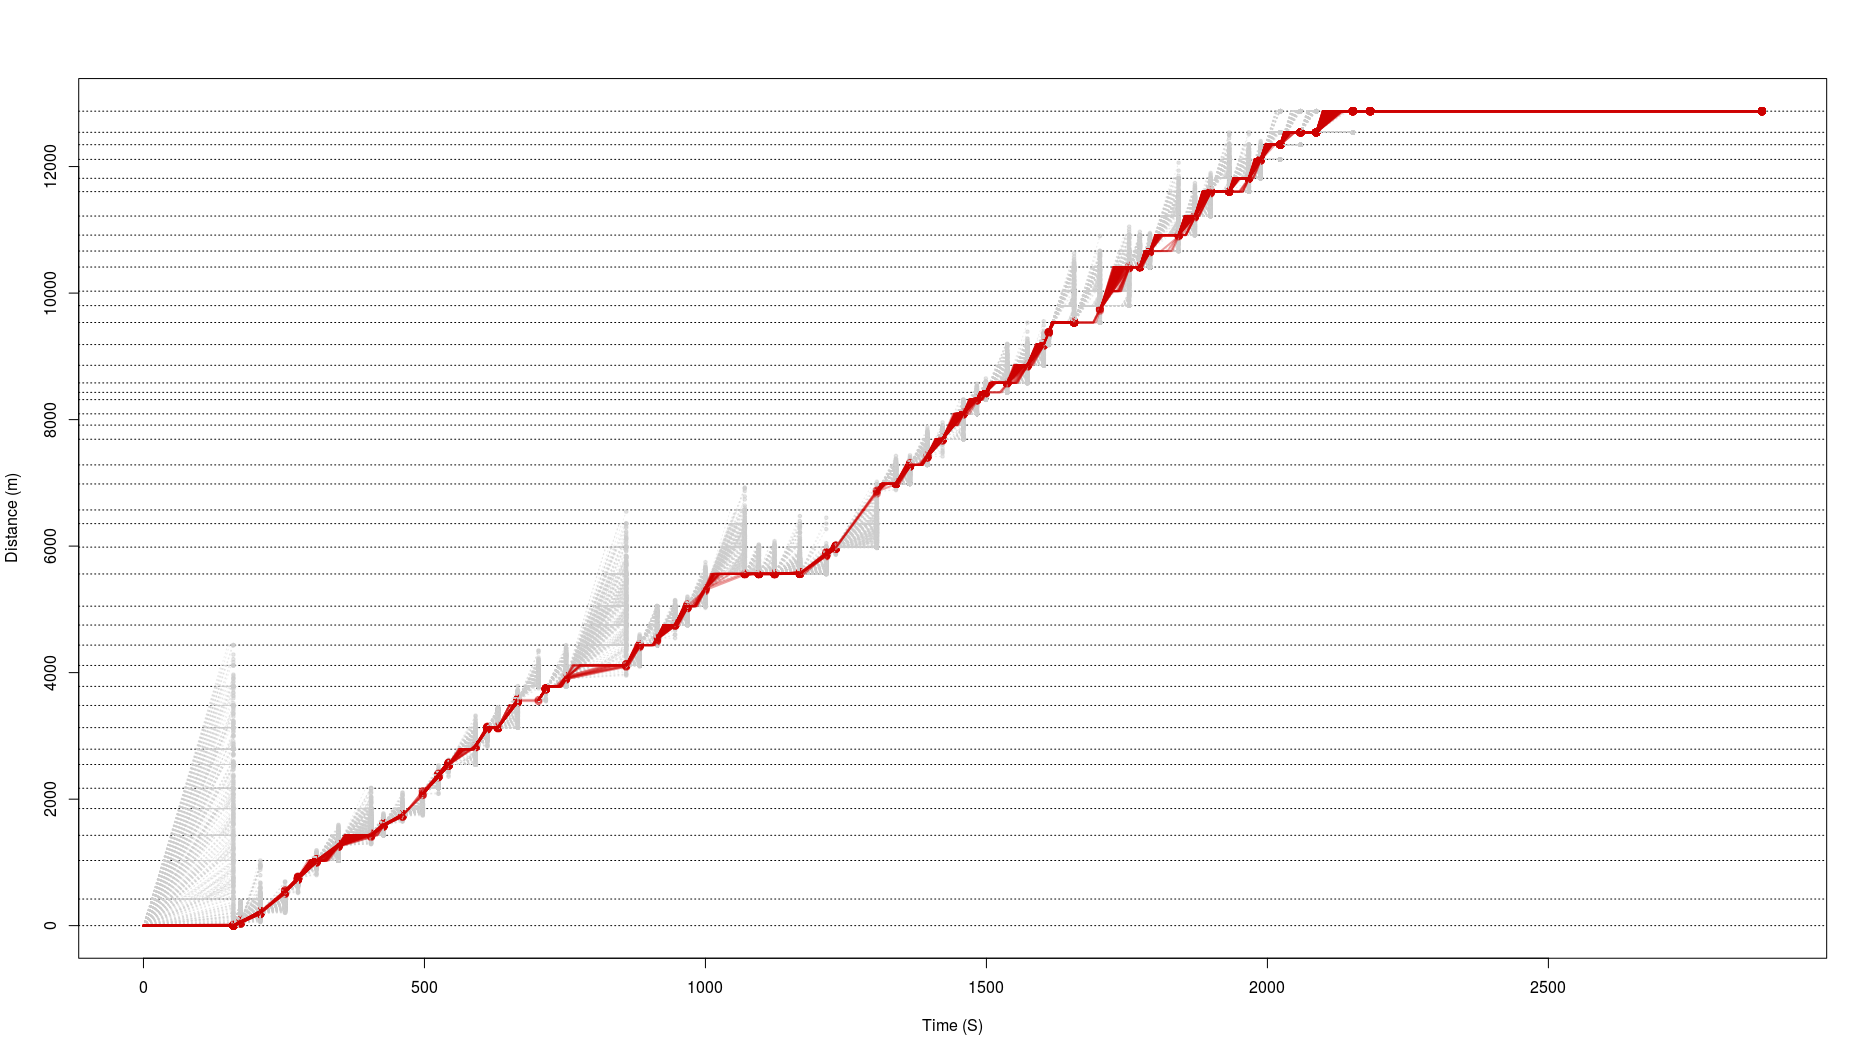
\includegraphics[width=\paperwidth]{figs/complete_route.png}
            };
        \end{tikzpicture}
     \end{frame}
}





\begin{frame}{Predicting Arrival Times}
  \onslide<+->

  \begin{itemize}[<+- | alert@+>]
  \item each future stop along a route; up to 1~hour in advance
  \item prediction model needs to be far more precise than state model
  \item can be computationally complex
    \begin{itemize}
    \item over 1000 buses at peak times
    \item each with up to 10, 20, 30?? stops ahead
    \end{itemize}
  \end{itemize}

  \onslide<+->
\end{frame}


\begin{frame}{Predicting Arrival Times: Schedule}
  \onslide<+->

  \begin{itemize}[<+- | alert@+>]
  \item each \emph{trip} has a \emph{schedule} with ``average'' arrival times
  \item given a particle's distance into trip, use scheduled travel time
    to predict ETA to a stop
    \begin{itemize}
    \item each particle has a distance into trip
    \item compare to scheduled ``arrival time'' at that ``distance''
    \item compute scheduled travel time to a stop
    \end{itemize}
  \end{itemize}


  \begin{overprint}
    \onslide<3>
    \centering
    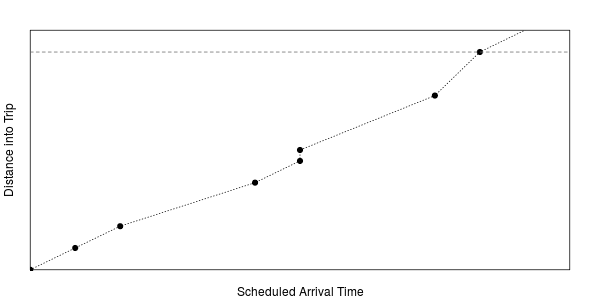
\includegraphics[width=0.8\textwidth]{figs/pred-sched-frame1.png}
    \onslide<4>
    \centering
    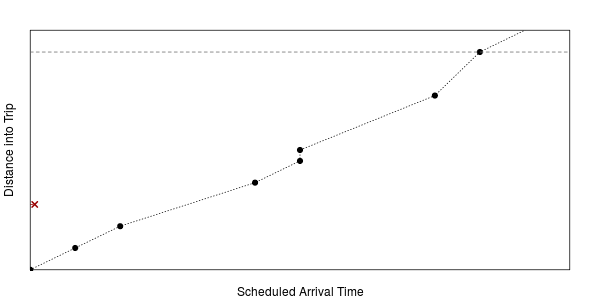
\includegraphics[width=0.8\textwidth]{figs/pred-sched-frame2.png}
    \onslide<5>
    \centering
    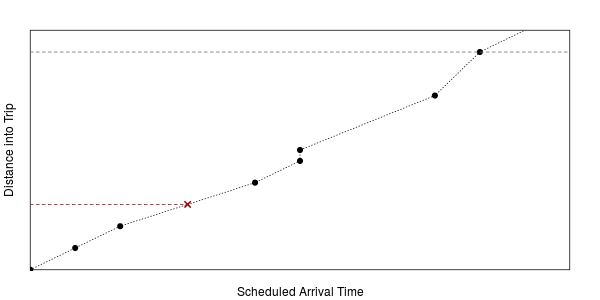
\includegraphics[width=0.8\textwidth]{figs/pred-sched-frame3.png}
    \onslide<6>
    \centering
    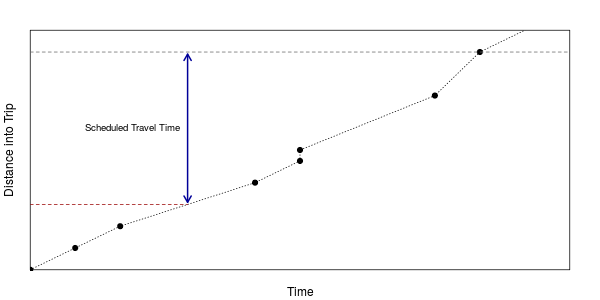
\includegraphics[width=0.8\textwidth]{figs/pred-sched-frame4.png}
  \end{overprint}

  \onslide<+->
\end{frame}


\begin{frame}{Predicting Arrival Times: Historical Data}
  \onslide<+->

  \begin{itemize}[<+- | alert@+>]
  \item replace schedule times with \emph{historical times}
  \item can build up models: trip, day of the week, time of day, etc
  \item historical data based on \emph{particle filter}: save summaries
  \item requires a lot of data (ANN, SVM, \ldots)
  \end{itemize}

  \onslide<+->
\end{frame}


\begin{frame}{Predicting Arrival Times: Realtime Data}
  \onslide<+->
  
  \begin{itemize}[<+- | alert@+>]
  \item have realtime data for 100's of buses around Auckland
  \item previous models use other buses traveling \emph{same route}
    (cite)
  \item propose: combining travel times/speed of \emph{all} buses in Auckland
    \begin{itemize}
    \item most up to date traffic/congestion data
    \item available \emph{now}, not after several weeks of data collection
    \end{itemize}
  \end{itemize}

  \onslide<+->
\end{frame}



\begin{frame}{Example with Predictions}
  Bus Route 274, Three Kings to Britomart


  \begin{overprint}
    \onslide<1>
    \centering
    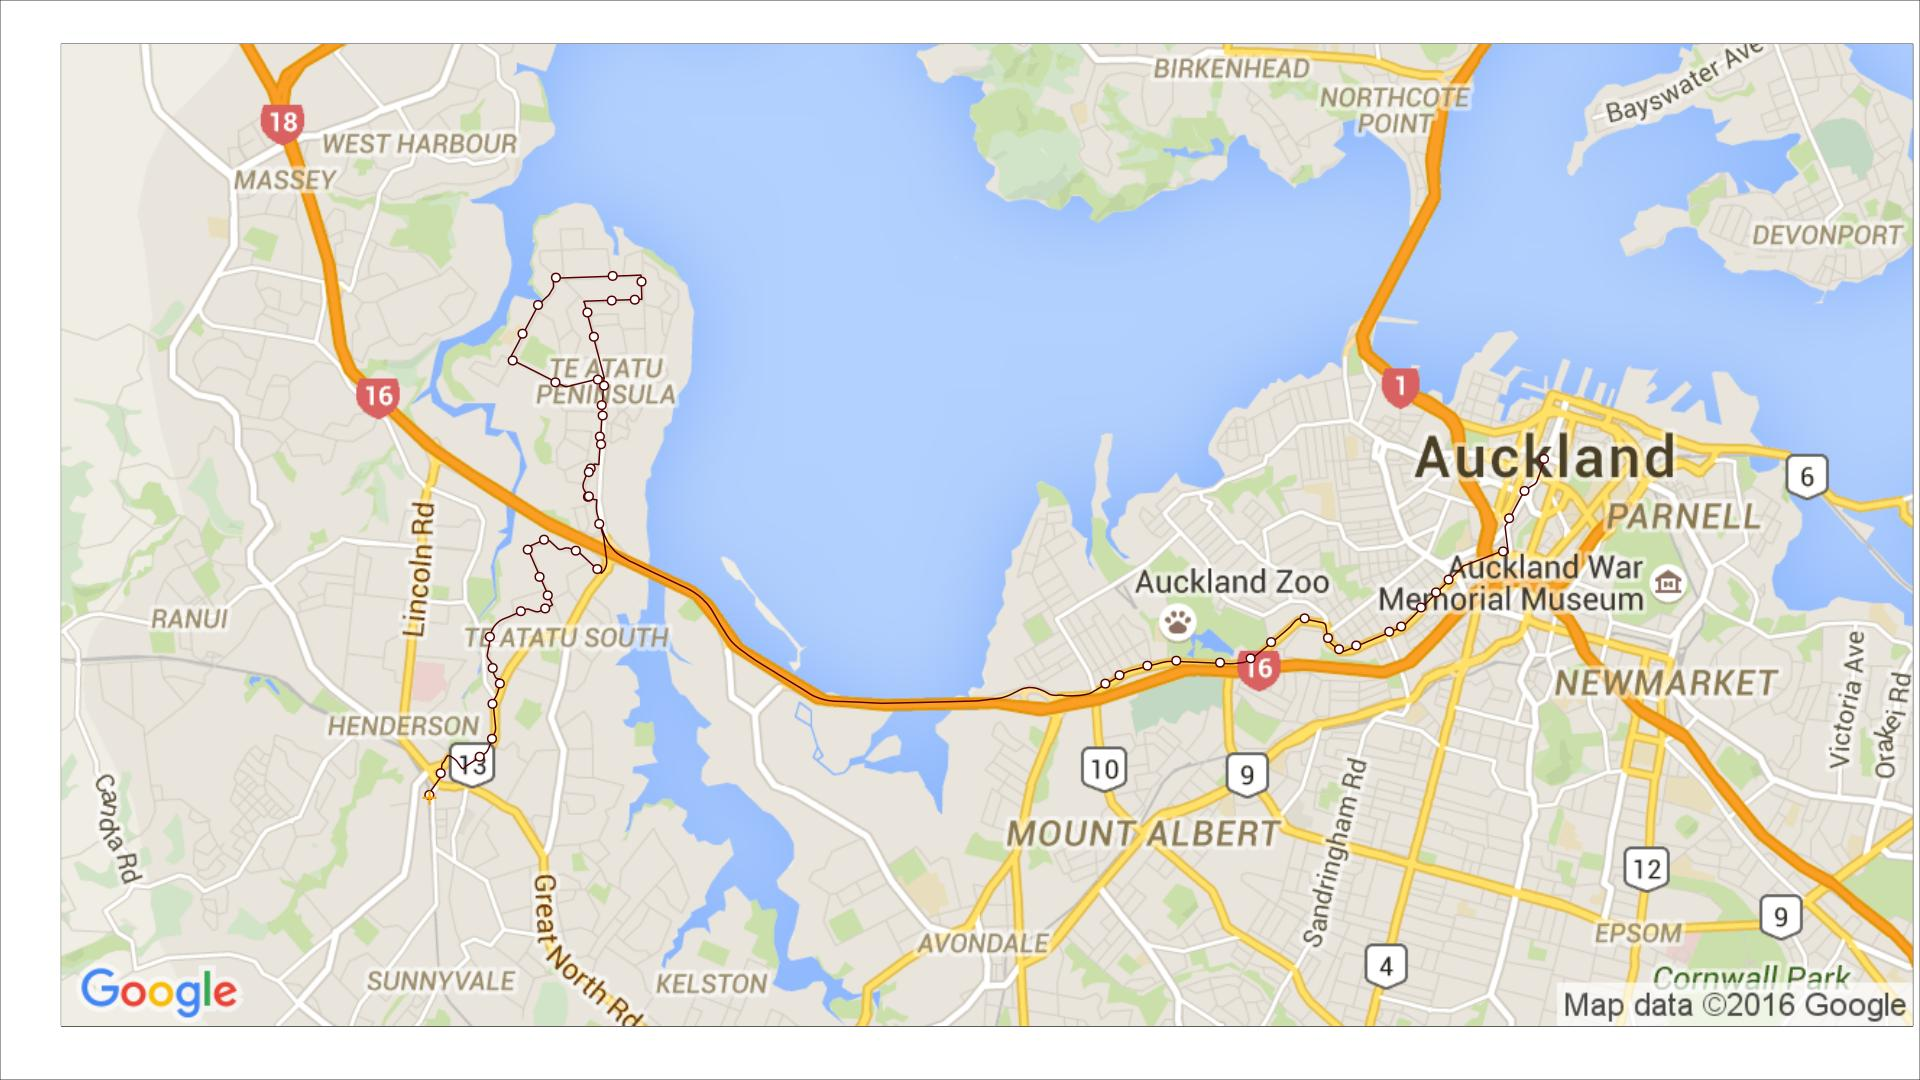
\includegraphics[width=1\textwidth]{figs/r274/TRIP5/particle_map001.jpg}

    \onslide<2>
    \vspace{2em}
    Particle Filter State Estimates and Transitions, 7~am trip
    \centering
    \includegraphics[width=1\textwidth]{figs/r274/TRIP5/distance_traveled.jpg}

    \onslide<3>
    \vspace{2em}
    ``Historical'' Data, 5:30~am, 6:00~am, 6.30~am, 6:50~am
    \centering
    \includegraphics[width=0.45\textwidth]{figs/r274/TRIP1/distance_traveled.jpg}
    \includegraphics[width=0.45\textwidth]{figs/r274/TRIP2/distance_traveled.jpg}\\
    \includegraphics[width=0.45\textwidth]{figs/r274/TRIP3/distance_traveled.jpg}
    \includegraphics[width=0.45\textwidth]{figs/r274/TRIP4/distance_traveled.jpg}

    \onslide<4>
    \vspace{2em}
    Arrival time prediction based on 4 previous trips
    \centering
    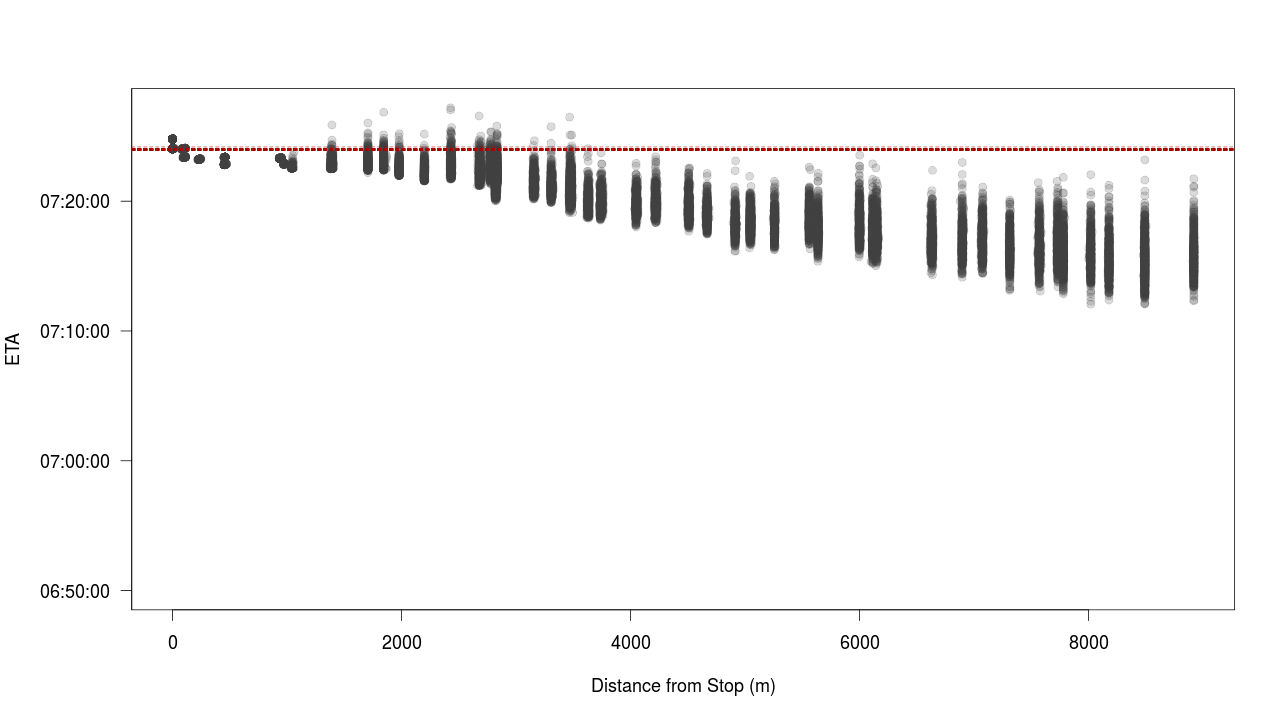
\includegraphics[width=1\textwidth]{figs/r274/TRIP5/arrival_last_hist.jpg}
  \end{overprint}
\end{frame}



\begin{frame}{Communicating Prediction}
  \onslide<+->

  \begin{itemize}[<+- | alert@+>]

  \item target audience: \emph{general public}
    
  \item inevitably going to be significant uncertainty in predictions, 
    particularly from a long way off

  \item need to convey \emph{distribution of particles} in an easy to understand manner

  \item \textbf{point estimates}:
    \begin{itemize}
    \item good for displays that can only fit a single digit
    \item for commuters, they imply ``accuracy''
    \end{itemize}
    
  \item \textbf{interval estimates}:
    \begin{itemize}
    \item standard practice for most statistical analyses
    \item but how to give a \emph{meaningful} interval to commuters?
      i.e., ETA: 3--7~mins = BETWEEN 3 and 7 minutes, with 100\% probability?
    \item also want non-symmetrical interval: being early to the bus stop is better than being late!
    \end{itemize}
  \end{itemize}

  \onslide<+->
\end{frame}




\begin{frame}[standout]
  Thank you!
\end{frame}


\end{document}
